\documentclass[11pt,a4paper]{article}
\usepackage{graphicx}
\usepackage{amsmath}
\usepackage{amssymb}
\usepackage{mathrsfs}
\usepackage{cancel}
\usepackage{graphicx}
\graphicspath{{Imagenes/}}
\usepackage[left=2.5cm,top=2.5cm,bottom=3cm,right=2.5cm]{geometry}



\begin{document}
\begin{center}
\textbf{REPORTE 1 DE AVANCE PROYECTO}\\
.\\
DRON INTELIGENTE
\end{center}

\begin{figure}[h]
\centering

\includegraphics[width=12.5cm]{upzmg.png} 
\end{figure}

\begin{center}
Maria de Lourdes Gomez Islas\\
Asencio de leon Agustín\\
Cruz Ramírez Jesús Osmar\\
González González eldrich johel\\
Calderón Hernández Richard\\
Partida López Ernesto Alonso\\
.\\
08-OCT-2019\\
Universidad Politecnica de La Zona Metropolitana de Guadalajara
\end{center}

\newpage 

\part{Planteamiento del problema}
El problema que se desea resolver con este proyecto es la inseguridad en los fraccionamientos mas vulnerables ante el crimen organizado y criminales de bajo nivel.
Los fraccionamientos como Chulavista o Santafé son muy vulnerables ante los crimenes, tanto así que ya se consideran de los fraccionamientos más peligrosos de Tlajomulco de Zuniga por lo cual se implementara un sistema de vigilancia de drones autónomos que monitorearan los policías en los  sectores en los que existe  falta de videovigilancia.
También se puede decir que el problema en el que ayuda sería hacia los fotógrafos ya que con este tipo de drones se pueden plasmar mejor las imágenes.

\section{Formular el problema}
Si el dron está volando en el aire y ve a alguien en peligro que pasaría?
La persona que en teoría esta monitoreando el dron o ese dron sería alertada del suceso y enviaria a la policía o a alguien que pueda resolver ese problema

¿El dron lo pueden usar otras personas?
Si, cualquier persona puede usar el dron desde un niño hasta un fotógrafo o para su uso específico que es la seguridad

\part{Objetivo general}
El objetivo general es construir un dron QUADCOPTER inteligente
que sea capas de detectar y seguir caras o
una bola roja.
Es un dron que nunca golpeara un árbol o
una pared y tiene funciones automáticas.
El dron contará con
*reconocimiento de rostros
*sistema de vuelo automático
*capacidad de evitar obstáculos por su
propia cuenta
*telemetría vía Bluetooth

\paragraph{Objetivo del proyecto:}


Este es el diseño de un dron totalemnte automatico e inteligente, los beneficios de este dron es, que ya no tendrá los pequeños accidentes que suelen ocurrir durante el proceso de vuelo los mas comunes son de golpear objetos tales como arboles y paredes, lo que planeamos a futuro con este proyecto es de darle una utilidad con el equipo de forma recreativa, brindando un dron que difilcilmete se dañara por choques y se perdera de forma menos comun, haciendolo un juguete de que dara divercion sin tanta preocupacion.


\part{Justificacion}

el proyecto se penso de forma que el dron tenga una resistencia mayor a un dron convencional, dado a que hay muchos testimonios y una problmatica comun entre las personas dueñas de drones que se pierdan o que se dañen al chocar de forma inesperada con algun objeto inamovible o animal incauto que este volando por la zona   \\
Lo elegimos por hecho de que es prácticamente algo complejo y automatizado,de lo 	ue se tiene conocimiento la mayoria de las personas gastan en varios drones con el mismo fin el a pesar de la experiencia de las personas, cual es perderse volandolos. 

\paragraph{Delimitacion:}


\begin{itemize}
\item Medicion Aprox. 45cm de distancia de ala a ala.
\item Peso Max. 2kg.
\item Altura de vuelo hasta 10m.
\item Tiempo de vuelo 30 hora antes de recargarce.
\item Alejamiento de el dispositivo de control 10m Aprox.
\end{itemize} 

\section{Posibles materiales y costos}

\begin{tabular}{|c|c|}
\hline
\textbf{Materiales} & \textbf{Costos}\\ \hline
Chasis o Frame & 700-800 \\ \hline
Motorizacion & 500 \\ \hline
PDB y Controladora & 250-2150 \\ \hline
Batería & 600 \\ \hline
Hélices & 200 \\ \hline
Emisora & 1000 \\ \hline
Equipo & 1600 \\ \hline
\end{tabular}



\section{Roles}

\begin{tabular}{|c|c|}

\hline
\textbf{Integrante} & \textbf{Rol} \\ \hline
Maria de Lourdes  & Encargada del Diseño \\ \hline
Ernesto Alonso & Encargado del Diseño \\ \hline
Jesús Osmar & Encargado de Impresion y Material \\ \hline
Hernández Richard & Encargado del Ensamblado \\ \hline
Maria de Lourdes & Calculos \\ \hline
Eldrich Johel & Parametros y Pruebas \\ \hline
Asencio de leon & Programacion \\ \hline
\end{tabular}

\subsection{Tiempos y Actividades}

\begin{figure}[h]
\centering
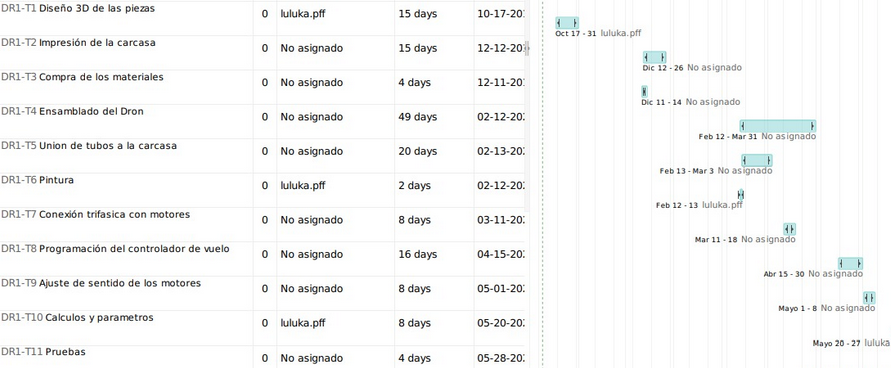
\includegraphics[scale=.5]{FFFFFFFFFF2}
\caption{Diagrama de GANTT}
\end{figure}


\newpage

\part{Explicacion de Aportacion de las materias}

\begin{tabular}{|p{5.5cm}|p{7cm}|}
\hline 
\textbf{Materias de 4to} & \textbf{Aportacion al proyecto} \\ \hline
\textbf{ingles 4} & Es indispensable saber el lenguaje de  ingles ya que es el lengueje universal para programar \\ \hline
\textbf{etica profesional} & Si hablamos de Etica, el valor de proteger al progimo a la familia y a la humanidad  se emplea en este proyecto ya que se lleva a cabo un sistema de vigilancia. \\ \hline
\textbf{estructura y propiedades} & Nos aporto la informacion indicada para el tipo de material a utilizar para la resistencia  del modelo \\ \hline
\textbf{programacion de perifericos} & Utilizar los aprendizajes de la materia para ser aplicador en la programacion rotatorio hacia los motores usando una Raspberry pi zero W \\ \hline
\textbf{S. E. de interfaz} & Hacer uso de un modelo trifasico para los motores conectado al programa y calculando la division requerida de tension.  \\ \hline
\textbf{PLC} & Este proyecto se llevara a cavo un dron controlado, con indicaciones seguido de sensores para hacer sus funciones. \\ \hline
\end{tabular}

\newpage
\begin{tabular}{|p{5.5cm}|p{7cm}|}
\hline 
\textbf{Materias de 5to} & \textbf{Aportacion al proyecto} \\ \hline
\textbf{ingles 5} & en la estructuración de palabras más profesionales dentro un formato de reporte o documento de elaboración con información de los proyectos a largo plazo 
Habilidades gerenciales: las pequeñas cualidades que se debe tener para poder liderear a un equipo de personas, las cuales de estas ya están dentro de la persona solo para desarrollar el rol de liderazgo, las cuales tiene que tener la capacidad de manejar estos tres grupos de personas en diferentes área las cuales son:  
Habilidades técnicas: Aquí se involucra el conocimiento y experticia en determinados procesos, técnicas o herramientas propias del cargo o área específica que ocupa.
Habilidades humanas:
Es la habilidad de interactuar efectivamente con la gente. Un gerente interactúa y coopera principalmente con los empleados a su cargo; muchos también tienen que tratar con clientes, proveedores, aliados, etc.
 \\ \hline
\textbf{Matemáticas ingeniería 1} & en determinar  áreas de regiones generales en el plano XY y volúmenes de sólidos irregulares. El resolver problemas de funciones vectoriales para contribuir a la solución de desplazaminetos de nuestro dron  \\ \hline
\textbf{Proceso de manufactura} & aportara con la investigación de mas tecnología, para obtener un mayor conocimiento en el avance de tecnologías de nuestro dron que vamos a desarrollar a lo largo de este año de elaboración. \\ \hline
\textbf{Sistemas digitales} & en diseñar sistemas lógicos digitales a través de principios de lógica booleana, técnicas de simplificación de circuitos, metodologías de diseño combinacional y secuencial. Desarrollo de soluciones de automatización de procesos productivos y servicios mediante la incorporación sinérgica de elementos mecánicos, eléctricos, electrónicos, control y sistemas robóticos para mejorar la productividad y calidad del proceso y producto. En proyectos de innovación e integración y automatización de procesos.  \\ \hline
\textbf{Sistemas neumáticos e hidráulicos} & Desarrollo de soluciones de automatización de procesos productivos y servicios, de elementos mecánicos, eléctricos, electrónicos, control y sistemas robóticos para mejorar la productividad y calidad del proyecto. En sistemas mecatrónicos y robóticos a procesos  de conexión eléctrica y electrónica, de acoplamiento y ensamble mecánico, programación y configuración de los elementos de control.  \\ \hline

\end{tabular}
\newpage
\begin{tabular}{|p{5.5cm}|p{7cm}|}
\hline 
\textbf{Materias de 6to} & \textbf{Aportacion al proyecto} \\ \hline
\textbf{Resistencia de materiales} & Está materia nos servirá para estudiar el comportamiento de los materiales de acuerdo a como este sometido el material que se va a utilizar, también nos servirá para saber que materiales usar en un momento dado, y para ver como reaccionará el materiales en condiciónes de calor,humedad, presión etc
 \\ \hline
\textbf{Cinematica de mecanismos} & está materia en si, servira mucho puesto que se hará un plano de todos los mecanismos o articulaciones, donde mediremos los grados de libertad y todos los posibles movimientos como en un ejemplo un brazo robotico  \\ \hline
\textbf{Control de motores eléctricos} & Esta materia Nos ayudará a controlar, y a saber utilizar los motores electricos, como hacerlos funcionar, donde hacerlos funcionar y como controlarlos, como utilizarlos , y cuáles motores utilizar, esta materia nos ayudará mucho en nuestro proyecto \\ \hline
\textbf{Automatización industrial } & Está materia funcionara para aprender a hacer sistemas automatizados, para hacer que nuestro proyecto tenga algún sistema que permita reaccionar por si solo, como algún grado de libertad,  o que se mueva por si solo, o que se apage y se encienda solo, que haga alguna acción por medio de un programa predeterminado  \\ \hline

\end{tabular}
\paragraph{Desarrollo del proyecto:}
Reunir los requisitos para empezar el proyecto, proponiendo ideas para concluirlo.

\cite{ruiperez2016diseno,}
\bibliographystyle{apalike}
\bibliography{ReporteBib}


\end{document}